\begin{transitionframe}{War induced structural changes in labor markets}
\begin{itemize}
    \item The Japanese federal bill in 1945 conscripted 28 million working men into their military (65\% of working pop.). 

    \begin{itemize}
        \item Labor markets suffered labor shortage.
        
        $\Rightarrow$ Introduced under-represented pop. into the workforce.
    \end{itemize}
    
    \
    \pause

    
    \item The public sector was partially exempt from drafting, but introduced female workers to cover the surge in public service tasks.
    
    \
    \pause

    \item However, most female workers exited their positions at the end of WW2.
 \end{itemize}
\end{transitionframe}

\begin{transitionframe}
\begin{figure}
    \centering
    \caption{Number of Female workers in the Tokyo Civil Service}
    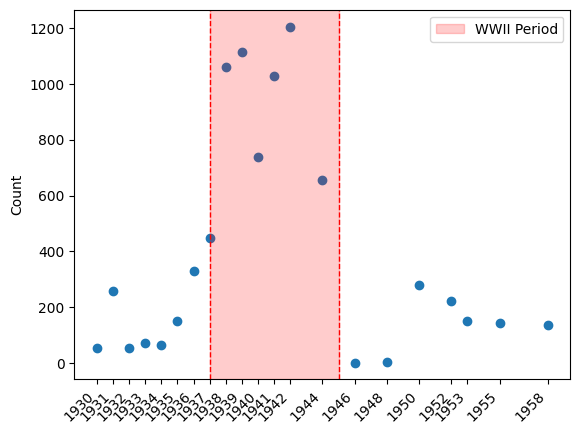
\includegraphics[width=\linewidth]{Background/FemaleEntry.png}
    \label{fig:time-series-figure}
    \hypertarget{Count}{}
    \hyperlink{Share}{\beamergotobutton{Share}}
\end{figure}
\end{transitionframe}